\documentclass{standalone}

\usepackage{xcolor}

\definecolor{myblue}{HTML}{377EB8}
\definecolor{myred}{HTML}{E41A1C}

\usepackage{tikz}
\usepackage{pgfplots}
\pgfplotsset{compat=newest}

\usepackage{lmodern}
\SetSymbolFont{letters}{bold}{OML}{cmbr}{bx}{it}
\renewcommand{\familydefault}{\sfdefault}

\usepackage{sansmathfonts}

\begin{document}
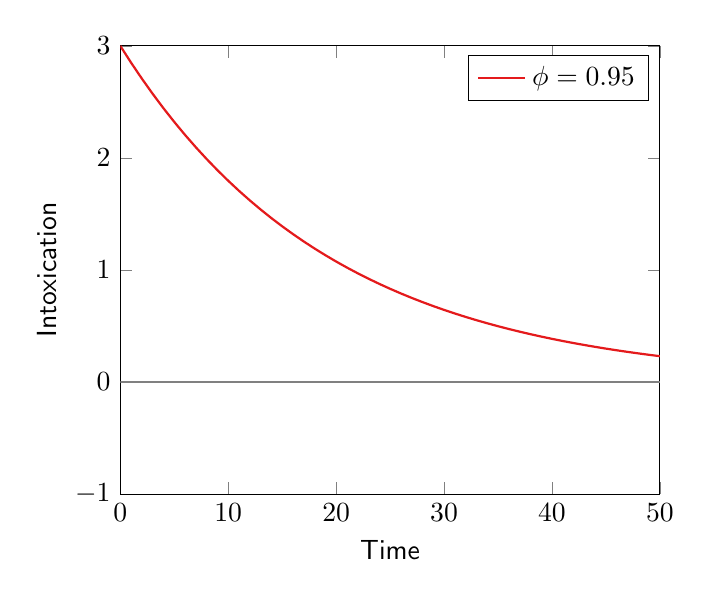
\begin{tikzpicture}
	\begin{axis}[
			xlabel={Time},
			ylabel={Intoxication},
			xmin=0, xmax=50,
			ymin=-1, ymax=3,
			xtick={0,10,20,30,40,50},
			ytick={-3,-2,-1,0,1,2,3},
			grid style=dashed,
		]		
		\addplot[
			color=myred,
            thick
		]
		coordinates {
			(0, 3)
			(1, 2.85)
			(2, 2.7075)
			(3, 2.572125)
			(4, 2.44351875)
			(5, 2.3213428125)
			(6, 2.205275671875)
			(7, 2.09501188828125)
			(8, 1.99026129386719)
			(9, 1.89074822917383)
			(10, 1.79621081771514)
			(11, 1.70640027682938)
			(12, 1.62108026298791)
			(13, 1.54002624983851)
			(14, 1.46302493734659)
			(15, 1.38987369047926)
			(16, 1.3203800059553)
			(17, 1.25436100565753)
			(18, 1.19164295537465)
			(19, 1.13206080760592)
			(20, 1.07545776722563)
			(21, 1.02168487886434)
			(22, 0.970600634921127)
			(23, 0.92207060317507)
			(24, 0.875967073016317)
			(25, 0.832168719365501)
			(26, 0.790560283397226)
			(27, 0.751032269227365)
			(28, 0.713480655765996)
			(29, 0.677806622977696)
			(30, 0.643916291828812)
			(31, 0.611720477237371)
			(32, 0.581134453375502)
			(33, 0.552077730706727)
			(34, 0.524473844171391)
			(35, 0.498250151962821)
			(36, 0.47333764436468)
			(37, 0.449670762146446)
			(38, 0.427187224039124)
			(39, 0.405827862837168)
			(40, 0.385536469695309)
			(41, 0.366259646210544)
			(42, 0.347946663900017)
			(43, 0.330549330705016)
			(44, 0.314021864169765)
			(45, 0.298320770961277)
			(46, 0.283404732413213)
			(47, 0.269234495792552)
			(48, 0.255772771002925)
			(49, 0.242984132452778)
			(50, 0.230834925830139)
			(51, 0.219293179538632)
			(52, 0.208328520561701)
			(53, 0.197912094533616)
			(54, 0.188016489806935)
			(55, 0.178615665316588)
			(56, 0.169684882050759)
			(57, 0.161200637948221)
			(58, 0.15314060605081)
			(59, 0.145483575748269)
			(60, 0.138209396960856)
			(61, 0.131298927112813)
			(62, 0.124733980757172)
			(63, 0.118497281719314)
			(64, 0.112572417633348)
			(65, 0.106943796751681)
			(66, 0.101596606914097)
			(67, 0.096516776568392)
			(68, 0.091690937739972)
			(69, 0.087106390852974)
			(70, 0.082751071310325)
			(71, 0.078613517744809)
			(72, 0.074682841857568)
			(73, 0.07094869976469)
			(74, 0.067401264776455)
			(75, 0.064031201537633)
			(76, 0.060829641460751)
			(77, 0.057788159387713)
			(78, 0.054898751418328)
			(79, 0.052153813847411)
			(80, 0.049546123155041)
			(81, 0.047068816997289)
			(82, 0.044715376147424)
			(83, 0.042479607340053)
			(84, 0.04035562697305)
			(85, 0.038337845624398)
			(86, 0.036420953343178)
			(87, 0.034599905676019)
			(88, 0.032869910392218)
			(89, 0.031226414872607)
			(90, 0.029665094128977)
			(91, 0.028181839422528)
			(92, 0.026772747451402)
			(93, 0.025434110078832)
			(94, 0.02416240457489)
			(95, 0.022954284346145)
			(96, 0.021806570128838)
			(97, 0.020716241622396)
			(98, 0.019680429541276)
			(99, 0.018696408064213)
		};
		\draw[gray] (0,0) -- (100,0);
		\legend{$\phi = 0.95$}
	\end{axis}
\end{tikzpicture}
\end{document}
